%---------------------------------------------------------------------
%
%                          Cap�tulo 5
%
%---------------------------------------------------------------------

\chapter{Implementation Study}

\begin{FraseCelebre}
\begin{Frase}
Time of your life
\end{Frase}
\begin{Fuente}
Thomas \& Guy-Manuel, Daft Punk
\end{Fuente}
\end{FraseCelebre}


\begin{resumen}
In this chapter, tasks related to the physical implementation of the platform are described. These tasks cover from the layout design, 3D modelling, and GERBER files generation, to the final components mounting on the . Decisions about components or layout designs, and final results are exposed.  
\end{resumen}



%-------------------------------------------------------------------
\section{Introduction}
%-------------------------------------------------------------------
\label{cap5:sec:introduction}
%------------------------------------------------------------------

Once the system is designed over a logic circuitry level, it is moment to build a \ac{PCB} design responsive to the developed schematics. This process includes the PCB dimmenssions, components placement, paths routing, silkscreens, etc. These tasks are achieved over the Altium Designer, same software described in Section \ref{cap4:sec:altiumDesigner}.

All the implementations share some common features regarding their layout designs. On the one hand, the used components will keep, whenever possible\footnote{Some components do not offer SMD packaging due to their electric properties.}, \ac{SMD} packaging. This technology gives a more reduced size and supports lower power ratings. Precissely, the \ac{SMD} package used for most of two-terminal components is the 0603 (1608 metric) size\footnote{1.6 mm x 0.8 mm (0.063 in x 0.031 in). Typical power rating for resistors are 0.1 watt.} Figure \ref{fig:cap5:smdsizes} shows a classification for two-terminal \ac{SMD} components in metrics and imperial units.

\begin{figure}
        \centering
                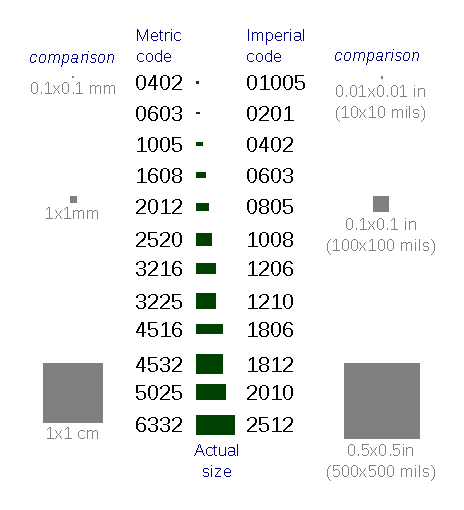
\includegraphics{Imagenes/Vectorial/Capitulo5/smdsizes}
        \caption{Two-terminal SMD packages classification.}
        \label{fig:cap5:smdsizes}
\end{figure}

All the created layouts are built over two-layer boards. Two layers are enough for our purposes since they allow to place the components in a sufficiently reduced area and power planes are not required. More layers, in addition, would increase significantly the board costs. 

For the paths routing process, some considerations are taken. Ground planes are placed to face noise reduction, this way a low impedance way is provided for the power signals. Moreover, parasitic \ac{EM} emissions are reduced. Power paths are width enough to support the supplied current flow.

Together with the layout deployment, Altium Designer offers the chance to embbed 3D models of each component, building up eventually a whole 3D model of the complete board. This tool was employed, and 3D models were rendered, obtaining a preview of the modules on advance to their materialization.

\ac{PCB} manufacturer, PCBCART\footnote{www.pcbcart.com} will produce the \ac{PCB}s from the outputed fabrication files. Final \ac{PCB} posses a 1.6 mm thickness, and copper layers are 35 $\mu$m thick. 

%-------------------------------------------------------------------
\subsection{Mounting}
%-------------------------------------------------------------------
Small package components, like the employed here, requires for precission tools to be mounted. Proper tweezers are helpful dealing with components. The soldering station used is a JBC AM 6000 ************REF, offering several soldering tips on the 1-4 mm diameter and useful tools as hot tweezers or desoldering accesories. Binocular loupe ************** WHATEVER ************ is essential for better precission. 

Components use to include at their datasheets guidelines about their surrounding layout, soldering tips, or mounting processes. They are reviewed and taken into account for the proccess.

The secuential mounting, and the existing firmware allow to carry through simple tests to ckeck proper functionality and detect errors. Actually, several corrections and adjustments were made during the mounting task.  

%-------------------------------------------------------------------
\section{Transceivers - $\mu$Trans 434/868}
%-------------------------------------------------------------------
\label{cap5:sec:transceivers}
%------------------------------------------------------------------

\figura{Vectorial/Todo}{width=0.4\textwidth}{fig:cap5:mtrans3dmodel}%
{$\mu$Trans 434/868 3D model.}

%-------------------------------------------------------------------
\subsection{Description}
%-------------------------------------------------------------------

This module was developed because of the non-existance of reduced size \ac{RI}s including the MRF49XA transceiver, so it must have a reduced size by definition. minimal spacing, track width, vias under the micro, pad to measure clock, ground plane

%SIZE, FIGURA

%holes to solder. footprint - porque FIGURA

\begin{table}[h]
\centering
\scalebox{0.7}{
\begin{tabular}{||c | c |||}
\hline \\
\hline \\
\hline \\
\hline \\

\end{tabular}
}
\caption{Component description for $\mu$Trans 434/868.%
         \label{tab:cap5:mtranscomponents}}
\end{table} 


%-------------------------------------------------------------------
\subsection{Layout}
%-------------------------------------------------------------------
%Referencias a ANEXO

%-------------------------------------------------------------------
\subsection{Testing}
%-------------------------------------------------------------------

%primero probado en FCD, errores detectados
%osciloscopio para sensar varias se�ales
%handshaking
%network detection
%data transmission reception

%-------------------------------------------------------------------
\subsection{Final Result}
%-------------------------------------------------------------------

%FOTOS

%-------------------------------------------------------------------
\section{Main Board - cognitiveNextGenerationDevice}
%-------------------------------------------------------------------
\label{cap5:sec:currentDevices}
%-------------------------------------------------------------------

\figura{Vectorial/Todo}{width=0.4\textwidth}{fig:cap5:cngd3dmodel}%
{cNGD 3D model.}

%-------------------------------------------------------------------
\subsection{Layout}
%-------------------------------------------------------------------

%-------------------------------------------------------------------
\subsection{Testing}
%-------------------------------------------------------------------

%-------------------------------------------------------------------
\section{Serial Communication Board - rs232SHIELD}
%-------------------------------------------------------------------
\label{cap5:sec:rs232shield}
%-------------------------------------------------------------------

\figura{Vectorial/Todo}{width=0.4\textwidth}{fig:cap5:rs2323dmodel}%
{rs232SHIELD 3D model.}

%-------------------------------------------------------------------
\subsection{Layout}
%-------------------------------------------------------------------

%-------------------------------------------------------------------
\subsection{Testing}
%-------------------------------------------------------------------

%-------------------------------------------------------------------
\section{Battery charger - chargerSHIELD}
%-------------------------------------------------------------------
\label{cap5:sec:chargerShield}
%-------------------------------------------------------------------

\figura{Vectorial/Todo}{width=0.4\textwidth}{fig:cap5:charger3dmodel}%
{chargerSHIELD 3D model.}

%-------------------------------------------------------------------
\subsection{Layout}
%-------------------------------------------------------------------

%-------------------------------------------------------------------
\subsection{Testing}
%-------------------------------------------------------------------

%-------------------------------------------------------------------
\section{Conclusions}
%-------------------------------------------------------------------
\label{cap5:sec:conclusions}
%-------------------------------------------------------------------


%------------------------------------------------------------------
%\section*{\NotasBibliograficas}
%-------------------------------------------------------------------
%\TocNotasBibliograficas

%Citamos algo para que aparezca en la bibliograf�a\ldots
%\citep{ldesc2e}

%\medskip

%Y tambi�n ponemos el acr�nimo \ac{CVS} para que no cruja.

%Ten en cuenta que si no quieres acr�nimos (o no quieres que te falle la compilaci�n en ``release'' mientras no tengas ninguno) basta con que no definas la constante \verb+\acronimosEnRelease+ (en \texttt{config.tex}).


%-------------------------------------------------------------------
%\section*{\ProximoCapitulo}
%-------------------------------------------------------------------
%\TocProximoCapitulo

%...

% Variable local para emacs, para  que encuentre el fichero maestro de
% compilaci�n y funcionen mejor algunas teclas r�pidas de AucTeX
%%%
%%% Local Variables:
%%% mode: latex
%%% TeX-master: "../Tesis.tex"
%%% End:
